%% 
%% Copyright 2019-2021 Elsevier Ltd
%% 
%% This file is part of the 'CAS Bundle'.
%% --------------------------------------
%% 
%% It may be distributed under the conditions of the LaTeX Project Public
%% License, either version 1.2 of this license or (at your option) any
%% later version.  The latest version of this license is in
%%    http://www.latex-project.org/lppl.txt
%% and version 1.2 or later is part of all distributions of LaTeX
%% version 1999/12/01 or later.
%% 
%% The list of all files belonging to the 'CAS Bundle' is
%% given in the file `manifest.txt'.
%% 
%% Template article for cas-dc documentclass for 
%% double column output.

\documentclass[a4paper]{cas-dc}
\newcommand{\figref}[1]{Fig.~\ref{#1}}
% If the frontmatter runs over more than one page
% use the longmktitle option.

%\documentclass[a4paper,fleqn,longmktitle]{cas-dc}

%\usepackage[numbers]{natbib}
%\usepackage[authoryear]{natbib}
\usepackage[authoryear]{natbib}

%%%Author macros
\def\tsc#1{\csdef{#1}{\textsc{\lowercase{#1}}\xspace}}
\tsc{WGM}
\tsc{QE}
%%%

% Uncomment and use as if needed
%\newtheorem{theorem}{Theorem}
%\newtheorem{lemma}[theorem]{Lemma}
%\newdefinition{rmk}{Remark}
%\newproof{pf}{Proof}
%\newproof{pot}{Proof of Theorem \ref{thm}}

\begin{document}
\let\WriteBookmarks\relax
\def\floatpagepagefraction{1}
\def\textpagefraction{.001}

% Short title
%\shorttitle{ASD diagnosis through deep learning}    

% Short author
%\shortauthors{Short author}  

% Main title of the paper
\title [mode = title]{Diagnosing autism spectrum disorders based on self-attention mechanism and dynamic functional connectivity}  

% Title footnote mark
% eg: \tnotemark[1]
%\tnotemark[1] 

% Title footnote 1.
% eg: \tnotetext[1]{Title footnote text}
%\tnotetext[1]{<Title footnote text>} 	% 文末注释

% First author
%
% Options: Use if required
% eg: \author[1,3]{Author Name}[type=editor,
%       style=chinese,
%       auid=000,
%       bioid=1,
%       prefix=Sir,
%     
%
%=0000-0000-0000-0000,
%       facebook=<facebook id>,
%       twitter=<twitter id>,
%       linkedin=<linkedin id>,
%       gplus=<gplus id>]

	\author[1]{Libiao Chen}



% Footnote of the first author
%\fnmark[Model building]

% Email id of the first author
\ead{chenlb318@emails.bjut.edu.cn}

% URL of the first author
%\ead[url]{<URL>}

% Credit authorship
% eg: \credit{Conceptualization of this study, Methodology, Software}
\credit{Methodology}

% Address/affiliation
\affiliation[1]{organization={Faculty of Information Technology, Beijing University of Technology},
            %addressline={}, 
            city={Beijing},
%          citysep={}, % Uncomment if no comma needed between city and postcode
            postcode={100000}, 
           % state={},
            country={China}}

\author[1]{Sizhe Wang}

% Footnote of the second author
\fnmark[1]

% Email id of the second author
\ead{wangsizhe@qq.com}

% URL of the second author
%\ead[url]{}

% Credit authorship
\credit{Software}

\author[1]{Zhenyu Wei}
\ead{weizhenyu@qq.com}
\credit{Software2}
\fnmark[1]

\author[1]{Yaoqing Zhang}
\ead{zhangyaoqing@qq.com}
\credit{Software3}

\author[1]{Mengzhu Luo}
\ead{luomengzhu@qq.com}
\credit{Software4}

\author[1]{Yin Liang}
\ead{liangyin@qq.com}
\credit{Software5}
% Corresponding author indication
\cormark[1]

% Address/affiliation
%\affiliation[2]{organization={Beijing University of Technology},
%	addressline={}, 
%	city={Beijing},
%	%          citysep={}, % Uncomment if no comma needed between city and postcode
%	postcode={100000}, 
%	state={},
%	country={China}}

% Corresponding author text
\cortext[1]{Corresponding author}
\cortext[1]{	
	This work was supported in part by the National Natural Science Foundation of China under Grant 61906006; and in part by the Beijing Municipal Science and Technology Project KM202310005026.}


% Footnote text
\fntext[1]{Second Author and Third Author contribute equally to this work.\\ 
}
%\fntext[2]{fntext 2}
% For a title note without a number/mark
%\nonumnote{}

% Here goes the abstract
\begin{abstract}
Autism spectrum disorder (ASD) is a severe developmental disorder that significantly impairs social abilities. Previous research has demonstrated impairments in functional brain connections in ASD patients. However,  existing research primarily relies on static functional connectivity and overlook critical information regarding temporal fluctuations. In this paper, we propose a novel strategy for diagnosing ASD based on a deep neural network and self-attention mechanism. Specifically, patient's dynamic functional connectivity (dFC) data were collected using sliding windows, and Kendall's rank correlation coefficient was utilized to extract the features. \textcolor{red}{By stacking multi-head self-attention layers and combining with feedforward neural networks, the proposed model can effectively extract higher-order features in spatial terms and stitch them together in temporal dimensions,while correlations across different temporal windows are also captured. We conducted extensive experiments on the ABIDE dataset to validate the performance of our model. Using ten-fold cross-validation, the proposed model achieved an average accuracy of 76.22\% and an AUC of 0.8132, while using inter-site cross-validation, the model achieved an average accuracy of76.71\% and an AUC of 0.7955, which outperformed similar studies in diagnosing ASD. Furthermore, we identified that the superior frontal gyrus and middle temporal gyrus are among the regions most affected in ASD, highlighting their importance for diagnosis and potential targets for intervention.Our model provides an effective approach for assisting in the diagnosis of ASD.}
\end{abstract}

% Use if graphical abstract is present
%\begin{graphicalabstract}
%\includegraphics{}
%\end{graphicalabstract}

% Research highlights
\begin{highlights}
\item A novel model employing the self-attention mechanism on dynamic functional connectivity is proposed for the classification of ASD. Based on the scores of feature rating, the most distinctive brain area connections are also displayed.

\item In this paper, sliding windows are used to acquire dynamic functional connectivity between brain regions, and Kendall rank correlation coefficients are employed for feature selection and as a basis for determining the most discriminative brain region connection. The multi-head self-attention mechanism was employed in conjunction with feedforward neural networks and residual networks to extract higher-order features from the data and discriminate ASDs.

\item This model obtained an average accuracy of 76.22\% and an AUC of 0.8132 on the ABIDE dataset, achieving excellent outcomes among similar studies. The superior frontal gyrus and middle temporal gyrus are identified as the brain regions most likely to cause ASD. 
\end{highlights}

% Keywords
% Each keyword is seperated by \sep
\begin{keywords}
 ASD\sep Self-Attention\sep dynamic FC\sep rs-fMRI \sep Kendall's rank correlation
\end{keywords}

\maketitle

% Main text
\section{Introduction}\label{Introduction}
Autism spectrum disorder (ASD) is a complex neurodevelopmental disorder characterized by social interaction deficiencies, communication deficits, restricted interests, and repetitive, stereotypical behaviors that typically appear in early childhood and can vary widely in severity and presentation. These deficiencies impact the learning and living of autistic patients, causing them to have considerable difficulties expressing their needs, comprehending others, and maintaining relationships, resulting in aberrant behaviors. In 2021, the CDC estimated that 1 in 44 U.S. children had been diagnosed with ASD (\cite{maenner2021prevalence}), highlighting the urgent need for effective diagnostic methods. However, current diagnostic approaches are limited to subjective symptomatological observations and clinical experiences, leading to variability in diagnosis across clinicians. In recent years, there has been growing interest in neuroimaging-based diagnostic approaches for ASD, as they can provide objective measures of brain structure and function that may be related to ASD symptoms and underlying pathology. By identifying aberrant connections between large-scale brain networks, neuroimaging methods can potentially improve early detection and diagnosis of ASD, and ultimately lead to more effective interventions and treatments.

Resting-state functional Magnetic Resonance Imaging (rs-fMRI) is a non-radioactive, non-invasive means of detecting functional brain activity. It depicts the variations in the Blood Oxygen Level Dependent (BOLD) signals that occur naturally when a subject is not engaged in a specific task. \cite{monk2009abnormalities} found that ASD altered the intrinsic connectivity of subjects' brain networks. \cite{woodward2015resting} found that neurological and psychiatric disorders are characterized by alterations in the interactions between rs-fMRI, suggesting that the entire brain should be considered a holistic network. To establish a network of functional brain connections, previous studies have typically used functional connectivity (FC) to quantify correlations between BOLD signals from different brain regions. This method have shown excellent results in various psychiatric disorders, such as Alzheimer's Disease(\cite{ju2017early}) and Major depressive disorder (\cite{zeng2012identifying}). Therefore, functional connectivity networks can be built using BOLD signals from all brain regions, and differences in connectivity between ASD patients and healthy individuals can be identified using statistical methods, which is proven to be effective. (\cite{woodward2015resting})(\cite{assaf2010abnormal})

Machine learning algorithms are widely employed for classification tasks due to their great efficiency and performance. \cite{abraham2017deriving} utilized support vector machine (SVM) on 871 samples and attained a cross-validation accuracy of 67\% between sites. \cite{ismail2022hec} proposed a hybrid ensemble-based classification (HEC) model, which obtained 80\% classification accuracy using random forest. \cite{song2019characterizing} obtained an average accuracy of 74.86\% on 235 samples using linear discriminant analysis(LDA).

Due to the single-layer structure of these traditional machine learning methods, it is difficult to acquire high-level information from complex features. Deep learning algorithms learn higher dimensional information by stacking layers to address these drawbacks. \cite{liang2021convolutional} proposed a novel convolutional neural network combined with a prototype learning (CNNPL) framework and got excellent results. \cite{xiao2018sae} divided the dataset for each subject into 30 independent components (IC) and used stacked autoencoder (SAE) to obtain 87.21\% accuracy on a small sample set. Long short-term memory (LSTM) were used by \cite{dvornek2017identifying} to obtain the temporal data from rs-fMRI and eventually achieved 68.5\% accuracy.

Although deep learning algorithms offers superior performance, most current research on ASD diagnosis ignores the dynamic changes in FC between brain regions. Instead, they assume that the subject's brain state remains constant during the test (5-30 minutes), which is proven to be inaccurate (\cite{calhoun2014chronnectome}, \cite{allen2014tracking}). To address this limitation, dynamic FC (dFC) based on the sliding window method has become a new research direction. The sliding window method divides the time series into many independent and overlapping windows, allowing for the evaluation of discrepancies between different windows and the capture of fluctuations in the sample's time series. \cite{savva2019assessment} investigates the effect of different window lengths on model performance. \cite{litjens2017survey} used convolutional neural network(CNN) and self-attention mechanism to achieve outstanding outcomes. Compared to static FC, dFC can capture the oscillations in the BOLD signal, which unquestionably contributes extra information to the discrimination of ASD.

%Methods for measuring correlations between brain regions are essential to building FC network. The most common way to measure the correlation between each pair of brain regions is using the Pearson correlation coefficient. In addition, Spearman's rank correlation coefficient (reference) and high-order FC(HOFC)(reference) were also used.

As time series are partitioned into several overlapping windows, the sliding window exacerbates the conflict among small sample sizes, high dimensionality and big parameters while simultaneously capturing more information. However, numerous recent investigations have demonstrated the sparseness of brain activity(\cite{ju2017early}). Thus, the network model is more susceptible to noise interference and overfitting. To reduce the interference of noise while acquiring more discriminative features, \cite{fredo2018diagnostic} employed conditional random forest to reduce the dimensionality of the FC matrix and used random forest to test the classification accuracy of each dimension. \cite{guo2017diagnosing} chose features from many trained sparse auto-encoders (SAE) with strong discriminating power. \cite{liang2021convolutional} ranked the characteristics using Kendall's rank correlation coefficient and retrieved more discriminative features without altering the raw data.

The self-attention (SA) mechanism is derived from the Transformer(\cite{vaswani2017attention}) in natural language processing. With its efficient performance and wide field of perception, the self-attention mechanism has been successfully applied to several fields. Recent research has focused on using SA to identify brain illnesses using rs-fMRI data(\cite{kim2022interpretable},\cite{zhang2022self}). The multi-head self-attention (MSA) mechanism computes the self-attention formulas in many subspaces in parallel and stitches the final results together in order to capture the data in distinct spaces.

%It has now replaced CNN to obtain superior results in various computer vision fields because it can combine global information and concentrate more on critical regions than CNN, which can only focus on local information within the convolution kernel. Meanwhile, parallelism makes SA more computationally efficient than RNN and LSTM. However, the self-attention mechanism lacks attention to temporal order, which means changing the input order does not affect the output. Transformer alleviates this problem by adding positional encoding information to the raw data without increasing the data's dimensionality.

This paper proposed a method for diagnosing ASD based on dFC and MSA mechanism. Initially, the raw data is partitioned into many independent but overlapping  windows on the time series using the sliding window method. For each window, the correlation between brain regions is assessed using Pearson correlation coefficients and constructed into feature vectors. Then the feature vectors of all windows are combined to form the input feature matrix for each sample. To overcome the problem of high dimensionality, feature extraction is performed using the Kendall rank correlation coefficient. The multi-head self-attention layers are used to capture correlations between different time windows and extract spatially higher-order features. Between the self-attention layers, the feedforward neural network structure further mixes and filters the features. The residual network before and after joining the feedforward neural networks accelerates model training and prevents gradient disappearance simultaneously. On the ABIDE dataset, the performance of the model is displayed and compared to other models using ten-fold cross-validation. Meanwhile, the generalization of the model is explained by inter-site cross-validation. Additionally, considering the feature ranking results of all windows together, we ranked the functional connectivity of brain regions most likely to cause autism. The main contributions of our work are as follows.
\begin{enumerate}[a)]
	\item A novel model employing the self-attention mechanism on dynamic functional connectivity is proposed for the classification of ASD. Based on the scores of feature rating, the most distinctive brain area connections are also displayed.
	\item After extracting features from the dFC data, stacked multi-headed self-attentive layers are employed to simultaneously capture the temporal correlation between all windows. For each window, the spatial features are downscaled in order to obtain more distinguishable features.
	\item This model obtained an average accuracy of 76.22\% and an AUC of 0.8132 on the ABIDE dataset, achieving excellent outcomes among similar studies. The superior frontal gyrus and middle temporal gyrus are identified as the brain regions most likely to cause ASD.
\end{enumerate}  

The rest paper is organized as follows. In the "Materials and Methods" section, we first describe how to preprocess raw data and generate dynamic functional connectivity using sliding windows. We then propose a feature reduction method based on Kendall's rank correlation coefficients and classify ASDs using a model based on the multi-head self-attention mechanism. In the "Result" section, we discuss the experimental results, compare them to other models, and offer the 20 functional connections that may contribute to ASDs. In the "Conclusion" section, we provide a paper summary.
% Numbered list
% Use the style of numbering in square brackets.
% If nothing is used, default style will be taken.


% Unnumbered list
%\begin{itemize}
%\item 
%\item 
%\item 
%\end{itemize}  

% Description list
%\begin{description}
%\item[]
%\item[] 
%\item[] 
%\end{description}  

% Figure
%\begin{figure}[<options>]
%	\centering
%		\includegraphics[<options>]{}
%	  \caption{}\label{fig1}
%\end{figure}




% Uncomment and use as the case may be
%\begin{theorem} 
%\end{theorem}

% Uncomment and use as the case may be
%\begin{lemma} 
%\end{lemma}

%% The Appendices part is started with the command \appendix;
%% appendix sections are then done as normal sections
%% \appendix
\section{Materials and Methods}\label{Materials and Methods}
\subsection{Data and preprocessing}
In this study, we use rs-fMRI data obtained from ABIDE database(\cite{craddock2013neuro}). The dataset comprises structural and static functional MRI data from 17 international imaging sites, with the goal of capturing and exchanging neuroimaging data from individuals with ASD and healthy controls. The dataset included 539 people with ASD and 573 healthy controls(HC), and a substantial amount of phenotypic data was also collected. However, due to variations in collection periods $T$ across sites, using the complete sample data to establish dynamic functional connections could result in different input sizes. Consequently, we dropped samples with too short a collection time and shortened those with a longer collection time. After taking into account the sample size and the time length of the sample, $T$ was set to 146. Additionally, We excluded samples with missing data. For each site following removal, sample information is shown in Table \ref{Table1}.

\begin{table}[]
\caption{Site information used in this paper}\label{Table1}
\begin{tabular*}{\tblwidth}{@{}cccc@{}}
\toprule
  \textbf{Sites} & \textbf{Size} & \textbf{Sample(ASD/HC)} & \textbf{Gender(M/F)} \\ % Table header row
\midrule
CALTHCH                 & 20                           & 8/12          & 14/6               \\
CMU                     & 1                            & 1/0           & 1/0                    \\
KKI                     & 34                           & 10/24          & 26/8                 \\
LEUVEN\_1               & 29                           & 14/15          & 29/0                \\
LEUVEN\_2               & 31                           & 13/18          & 24/7                \\
NYU                     & 166                          & 71/95          & 132/34              \\
OLIN                    & 25                           & 14/11          & 20/5                \\
PITT                    & 32                           & 17/15          & 25/7                \\
SBL                     & 8                            & 3/5           & 8/0                \\
SDSU                    & 27                           & 9/18          & 21/6                \\
STANFORD                & 36                           & 17/19          & 28/8                \\
TRINITY                 & 43                           & 21/22          & 43/0                \\
UM\_1                   & 82                           & 36/46          & 59/23               \\
UM\_2                   & 31                           & 12/19          & 29/2                 \\
USM                     & 61                           & 38/23          & 61/0                \\
YALE                    & 48                           & 22/26          & 34/14               \\
TOTAL                   & 674                          & 306/368         & 554/120            \\
\bottomrule
\end{tabular*}
\end{table}
To facilitate further research and expansion, we used the preprocessing version of ABIDE dataset and use Anatomical Automatic Labeling (AAL) template to classify brain regions(\cite{rolls2015implementation}). The AAL template, provided by the Montreal Neurological Institute (MNI), divides the whole brain region of interest (ROI) into 116 regions, with 90 belong to the brain and 26 to the cerebellum. The sample data for each subject is arranged as a table of $T\times R$, where $R$ is the number of ROI. Each value represents the average BOLD signal strength of all the voxels in a given ROI at that particular time.

The BOLD signal in the brain region will be erroneous during data collection due to subject head movement and instrument error. Thus the data must be pre-processed. The main steps include Time correction, Head motion realignment, Coregister, Normalize, Smooth, Detrend, Filter.

\begin{figure*}[t]
	\centering
	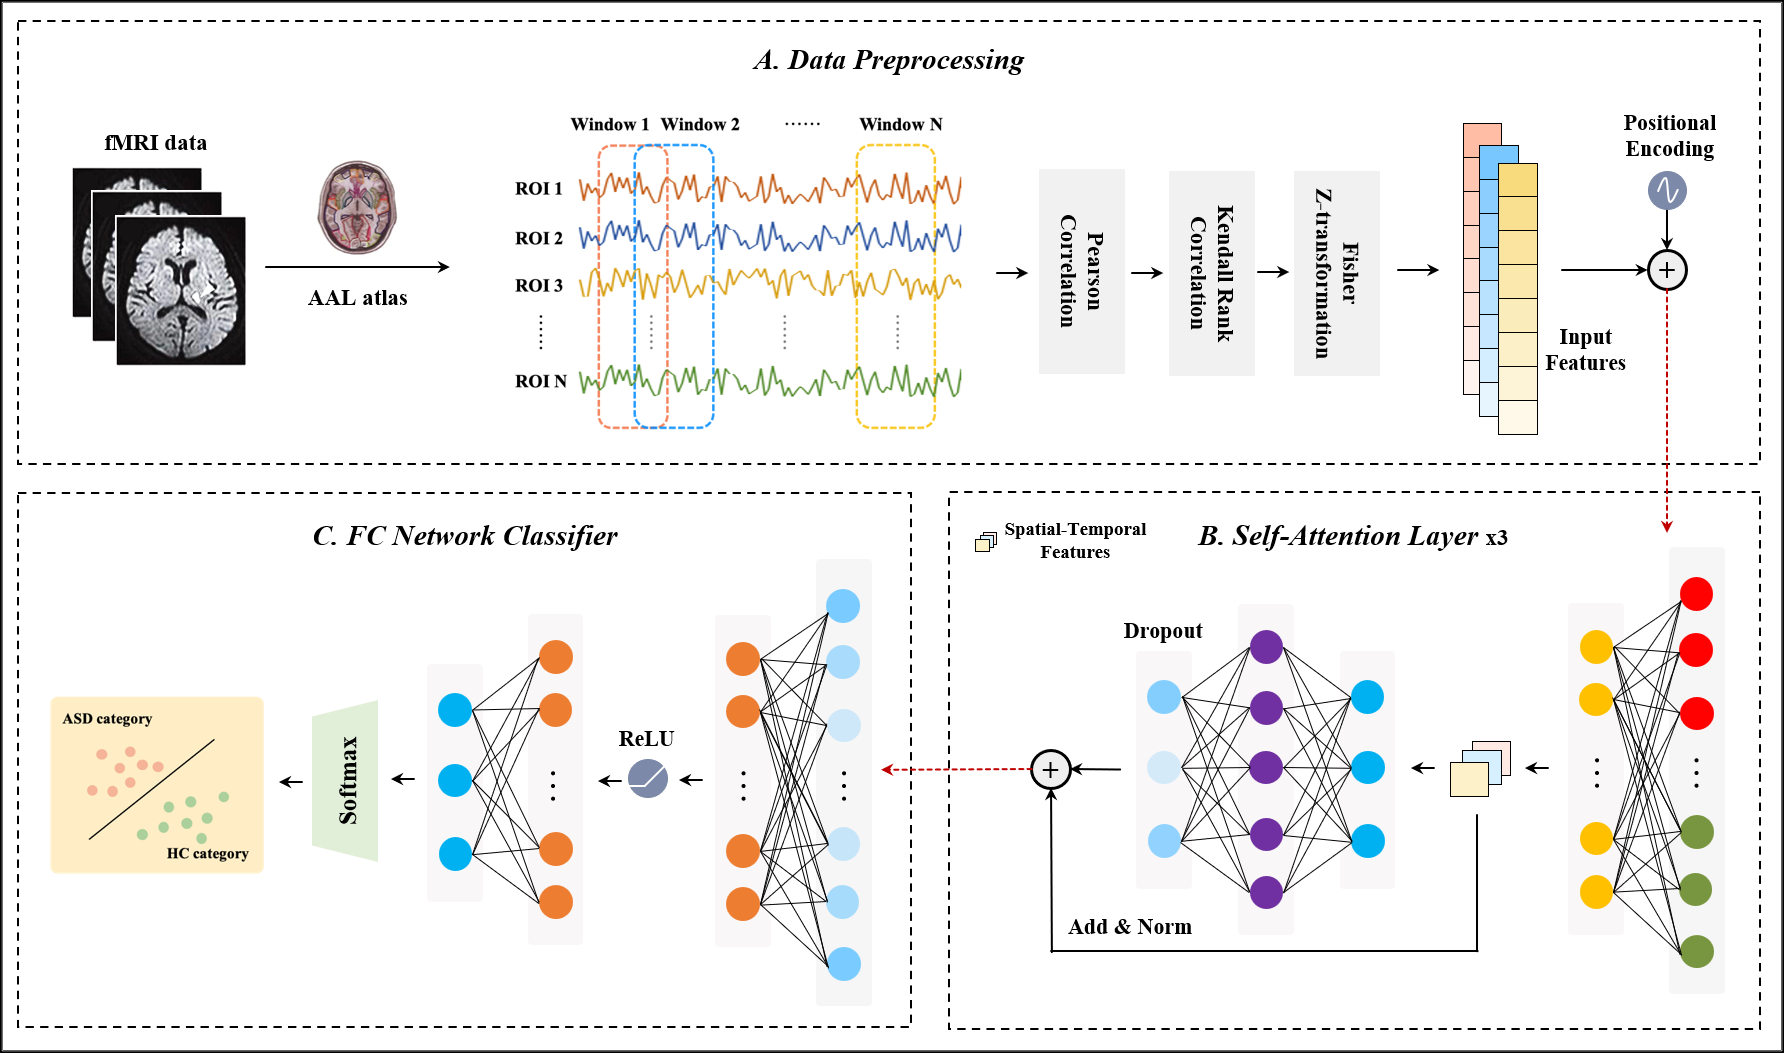
\includegraphics[width=\textwidth]{imgs/model.png}
	\caption{Flowchart of this paper. Box A shows dynamic functional connection acquisition. Box B shows feature extraction and normalization. Box C shows stacking multi-head self-attention layers with fully connected layers for classification. Box D shows the multi-head self-attention layer structure.}
	\label{fig1}
\end{figure*} 

\subsection{Construction of Brain Functional Network}
The complete flow chart of the model is shown in \figref{fig1}. This section will explain how to generate dynamic brain functional connectivity networks using preprocessed data. 
\paragraph{Silding Windows Method}~{}
\newline
\indent Initially, assume that a window of fixed length $l$ moves through the time series of data at a constant step $s$. The window partitions the entire time series into many overlapping but mutually distinct subsequences. The sliding window method necessitates the selection of parameters such as window length and window step beforehand. The window length determines the balance between temporal resolution and estimating precision(\cite{savva2019assessment}). Smaller window sizes are more sensitive to changes in time, but they add more noise, exacerbating the challenges of small sample sizes and high dimensionality. Based on previous research, we set the window length $l$ = 30 and the step size $s$ = 1, the preprocessed data is divided into $N$ separate windows,where $N = \left \lfloor \frac{T - l}{s} \right \rfloor + 1$
\paragraph{Pearson's Correlation Coefficient}~{}
\newline
\indent Brain connections create a sophisticated network that enables a variety of high-level tasks. Pearson's correlation coefficient is widely used to establish functional connectivity between brain regions. It quantifies the linear relationship between two variables, in this case the BOLD signal time series of two brain. If the linear correlation is strong, it indicates that both brain regions are reaching an active state at the same time and are likely to be involved in a common functional task.(\cite{ju2017early}).

Pearson's correlation coefficient assumes that the data follow a normal distribution so we conducted the Shapiro-Wilk test on randomly selected regions of the brain for each sample to assess whether the data followed a normal distribution. The results indicated that $P=0.421\pm 0.295>0.05$ and $W=0.989\pm 0.004$, which indicate that we could not reject the null hypothesis at the 0.05 level of significance, and the time series followed a normal distribution.Testing this assumption is important because it ensures that the results of the correlation analysis are reliable and interpretable.

For each window $W_n$, We define $x_{i}(t)$,$x_{j}(t)$ as the BOLD signals of two brain regions $i$ and $j$ at time point $t$($t = 1,2,...,l$).The $FC_{ij}$ can be defined as,
\begin{equation}
	FC_{ij}=\frac{\sum_{t=1}^{l}(x_{i}(t)-\bar{x_{i}})(x_{j}(t)-\bar{x_{j}})}{\sqrt{\sum_{t=1}^{l}(x_{i}(t)-\bar{x_{i}})^2}\sqrt{\sum_{t=1}^{l}(x_{j}(t)-\bar{x_{j}})^2}}
\end{equation}
where $\bar{x_{i}}$ and $\bar{x_{j}}$ represent the mean of rs-fMRI in brain regions $i$ and $j$. For AAL with 116 ROIs, the calculation between every two regions will end up with $F$ features, where $F=6670$ for AAL. Each window's feature vector contains all 6670 features. Each sample's feature matrix is created by merging the feature vectors of all windows. The shape of the feature matrix can be expressed as $N\times F$.
\subsection{Feature Ranking by Dynamic Kendall Rank Correlation}
Compared with static FC, dFC providesa more informative representation of brain activity while making the problem of high feature dimensionality more significant. Reducing the number of features by retaining more discriminative features can effectively reduce redundant noise in the data and improve computing efficiency. In this paper, we used the Kendall rank correlation coefficient, which measures the relevance of each feature with the classification by a distribution-free test of independence between two variables(\cite{zeng2012identifying}). We apply it separately to each window and combine the rating results to determine the final set of selected features. 

Assume that $m$ and $n$ correspondingly represent the number of ASD patients group and HC group. For the $i$-th window of all samples, Let $z_{jk}$ denote the $j$-th feature of the $k$-th sample and $y_i$ denote the class label of this sample. For $z_{jp}$ from the ASD patient group and $z_{jq}$ from the HC group, the $i$-th window's Kendall tau correlation coefficient of the functional connectivity feature $j$ can be defined as:
\begin{equation}
	\tau_{ij} = \frac{n_c - n_d}{m \times n}
\end{equation}
where $n_c$ and $n_d$ denote the numbers of concordant and discordant pairs. It is a concordant pair when
\begin{equation}
	sgn(z_{jp} - z_{jq}) = sgn(y_p-y_q)
\end{equation}
where sgn() is a signum function. Correspondingly, it is a disconcordant pair when
\begin{equation}
	sgn(z_{jp} - z_{jq}) = -sgn(y_p-y_q)
\end{equation}

The absolute value of each $\tau_{ij}$ reflects the ability of feature $j$ to detect ASD in the $i-th$ window, with a higher absolute value indicating a stronger discriminating power. To represent the combined discriminative capacity of feature $j$ across all windows, we average its correlation coefficients $\tau_{ij}$ over all windows, yielding $\tau_{j}$, which can be expressed as:
\begin{equation}
	\tau_{j} =  \frac{1}{N}\sum_{i=1}^{N}\tau_{ij}
\end{equation}

By ranking the $\tau_{j}$ values from highest to lowest, we select the top $C$ ($C\leq F$) features that are most informative for detecting ASD. The value of $C$ is chosen based on the sparsity of functional brain connections, with a smaller $C$ reducing the effect of noise but potentially leading to a loss of meaningful information. 

Recalling the method of calculation of features,it actually represents the correlation between the BOLD signals of two brain regions. Thus higher ranked features represent the connections between the corresponding two brain regions more likely to cause ASD.
\subsection{Classification based on Multi-Head Self-Attention}
\paragraph{Positional Encoding}~{}
\newline
\indent Self-attention mechanisms can help models understand global relationships between inputs and identify essential information by assigning different weights to inputs. However, while its parallelism increases the efficiency of the model's operations, it disregards the order of the model's inputs, which means changing the order of the model's inputs has no effect on the model's output(\cite{litjens2017survey}). It can lead to a loss of temporal information, especially when the inputs are continuous time windows.

To tackle this issue, we employ the same position encoding strategy as Transformer(\cite{vaswani2017attention}), appending position information to the data before it enters the self-attention layer. Specifically, we define each independent window as $n_i(i=1,2,..., N)$ and each window's feature vector index as $c_j(j=1,2..., C)$. We use sine and cosine functions with different frequencies to determine the positional encoding $PE$, which can be represented as,
\begin{equation}
	PE_{(c_i,2k)}=sin(c_i/10000^{2k/C})
\end{equation}
\begin{equation}
	PE_{(c_i,2k)}=cos(c_i/10000^{2k/C})
\end{equation}
Where $k(k<\frac{j}{2})$ is used to map to index $j$. Then, $PE$ is added to each sample's data to provide positional encoding information without expanding the data's dimensions.

\paragraph{Self-Attention Layer}~{}
\newline
\indent The self-attention layer is a crucial component of our model, which takes $N$ windows as input, with each window having a dimension of $C$. The vector $I = (I_0, I_1,..., I_N)$ is first fed into the self-attention layer, where three matrix $Q$,$K$,$V$ are defined as
\begin{equation}
	Q = IW_Q
\end{equation}
\begin{equation}
	K = IW_K
\end{equation}
\begin{equation}
	V = IW_V
\end{equation}
Here, $W_Q$, $W_K$ and $W_V$ are learnable weight matrices.The weights of the input vectors are then defined as
\begin{equation}
	\alpha = Softmax(\frac{QK^T}{\sqrt{d_k}})
\end{equation}
where $d_k$ is the dimension of the K matrix,and the Softmax function is used to normalize the weights so that they sum to 1. Finally, the output matrix O is defined as
\begin{equation}
	O = \alpha V
\end{equation}

Due to the complexity of brain functional connectivity, we incorporated the multi-head self-attention layer to obtain rich information on functional connectivity. The multi-head self-attention layer creates $H$ subspaces, executes the self-attention function on each subspace in parallel, and then combines the results of all subspaces as output.

Furthermore, to extract higher-order features while reducing the number of parameters, we stack multiple layers of the multi-head self-attention layer while making the dimension $d_v$ of the matrix $V$ smaller than the dimension $d_{qk}$ of matrices $Q$ and $K$ for dimensionality reduction. The output dimension of the multi-head self-attention layer can be expressed as $N\times Hd_v$. With the above structure, the model can extract more discriminative spatial features while capturing temporal correlations between windows. In this experiment, we stacked three layers of multi-head self-attention layer. The amount of features per window for each output layer is 500, 200, and 50.

We incorporate feedforward neural networks between the multi-head self-attention layers to achieve nonlinear transformation of features. First, the output of the self-attention layer was transferred to a higher dimension using a linear projection layer, followed by a ReLU activation function to combine features and produce deeper associations. Then, the higher-dimensional output was reduced back to the original dimension using another linear projection layer to eliminate combinations with low discriminatory power.

To avoid the gradient vanishing and speed up the model's training, we added a residual network to the feedforward neural network. Additionally, a Dropout layer was utilized to prevent overfitting of the model. The flow chart of the algorithm is shown in Algorithm 1.

Following these operations, the data was reduced to two dimensions by the fully connected layer, and the model output was generated by Softmax. The loss function used in the model is the cross-entropy loss function combined with the L2 regularized loss function. The optimizer used is SGD.

\begin{table}[]
	\tabcolsep=1cm
	\label{algorithm}
	\begin{tabular*}{\tblwidth}{@{}lllll@{}}
		
		\toprule
		\textbf{Algorithm 1} Multi-Head Self-Attention Network  \\ \midrule
		\textbf{Input}: Input matrix $I$                           \\
		\textbf{Output}: Result probability $O$                    \\
		Initialization: shared weights $W_Q$,$W_K$,$W_V$           \\
		hyperparameters: $H$,$d_{k}$,$d_v$,$max\_layer$         \\
		\\
		1:  ~~\textbf{while} epoch < max\_epochs \textbf{do}                     \\
		2:  ~~\quad \textbf{for} $l \leftarrow  1$ \textbf{to} max\_layers \textbf{do}                     \\
		3:  ~~\qquad \textbf{for} $h \leftarrow 1$ \textbf{to} $H$ \textbf{do}                               \\
		4:  ~~\qquad \quad $Q_{h,l}=IW_Q$,$K_{h,l}=IW_K$,$V_{h,l}=IW_V$                       \\
		5:  ~~\qquad \quad $\alpha = Softmax(QK^T / \sqrt{d_k})$			\\
		6:  ~~\qquad \quad $Z_{h,l} = \alpha V$							\\
		7:  ~~\qquad \textbf{end for}                                       \\
		8:  ~~\qquad $Z_l = Concatenate(Z_{1,l},Z_{2,l},...,Z_{h,l})$            \\
		9:  ~~\qquad $U_l = ReLU(W_{1,l}Z_l)$                              \\
		10:\qquad $H_l = W_{2,l}U_l$                                    \\
		11:\qquad $I\leftarrow H_l$                                          \\
		12:\quad \textbf{end for}                                      \\
		13:\quad$O = Softmax(WH_l)$                                      \\
		14:\textbf{end while}								\\
		15:return O                                     \\
		\bottomrule
	\end{tabular*}
\end{table}

\section{Result}
In this section, we analyze the effect of the number of features chosen and the number of heads of the multi-head self-attention layers, compare the method described in this research to previous models, and demonstrate the brain area connections most likely to induce ASD.
\subsection{Impact of feature numbers and head numbers to classification results}
Due to the sparsity of brain connections and the high dimensionality, the number of features chosen becomes a key determinant of classification outcomes. In order to determine the optimal value for the number of features, we trained the model utilizing the top 100, 512, 1024, 1600, and 6670 Kendall features, respectively, and chose accuracy, sensitivity, specificity and AUC as the evaluation indicators. The conclusive results are shown in Table \ref{Table2}. 

We can see that the model performs best with 1024 features, and its accuracy increases by 8.92\% compared with no feature reduction, indicating that there is a great deal of noise in the raw data and that feature extraction is essential. To demonstrate the dependability of feature ranking, we randomly picked 1024 features for testing, and the results demonstrate that Kendall can not only minimize the data dimensionality but also select the most discriminative features in a very effective way.
\begin{table}[]
	\caption{Experimental results using 100, 512, 1024, 1600, and 6670 features as model inputs,(r) means random}\label{Table2}
	\begin{tabular*}{\tblwidth}{@{}ccccc@{}}
		\toprule
		\textbf{Number}& \textbf{Accuracy} & \textbf{Sensitivity} & \textbf{Specificity} & \textbf{AUC} \\ % Table header row
		\midrule
		100                                     & 0.7090              & 0.6453                & 0.7651                 & 0.7664           \\
		512                                     & 0.7448              & \textbf{0.7112}       & 0.7759                 & 0.8080           \\
		1024                                    & \textbf{0.7622}     & 0.6554                & 0.8458                 & \textbf{0.8132}  \\
		1024(r)                                 & 0.6045              & 0.2869                & 0.8426                 & 0.6162           \\
		1600                                    & 0.7463              & 0.6253                & 0.8490                 & 0.7930           \\
		6670                                    & 0.6716              & 0.4482                & \textbf{0.8583}        & 0.7034 \\
		\bottomrule
	\end{tabular*}
\end{table}

We also investigated the effect of the number of heads $H$ on model performance in the multi-head self-attention layers, and the experimental results are shown in Table \ref{Table3}.The model performed best at $H$ = 6, indicating that the functional brain connections contain a wealth of information that can be effectively captured by the multi-head self-attention layer. When the number of heads exceeds six, it becomes increasingly difficult for the number of samples to support the training of a high number of parameters, resulting in a decline in the model's efficacy.
\begin{table}[]
	\caption{Experimental results using 1,2,4,6,8 heads in multi-head self-attention layers}\label{Table3}
	\begin{tabular*}{\tblwidth}{@{}ccccc@{}}
		\toprule
		\textbf{Number}& \textbf{Accuracy} & \textbf{Sensitivity} & \textbf{Specificity} & \textbf{AUC} \\ % Table header row
		\midrule
		1                            & 0.7343                & 0.6465                   & 0.8123                   & 0.7996           \\
		2                             & 0.7507                & \textbf{0.6751}          & 0.8177                   & 0.8022           \\
		4                             & 0.7358                & 0.6190                   & 0.8315                   & 0.8028           \\
		6                             & \textbf{0.7622}       & 0.6554                   & \textbf{0.8458}          & \textbf{0.8132}  \\
		8                             & 0.7343                & 0.6039                   & 0.8451                   & 0.8040      \\
		\bottomrule
	\end{tabular*}
\end{table}
\subsection{Results presentation and model comparison}
We employed the k-fold cross-validation method to maximize the use of samples for model testing, which is commonly employed on small sample datasets. Specifically, we divides all samples into $k$ folds, selects $k-1$ folds as the training set and 1 fold as the test set for training, and repeats this process $k$ times to classify each fold as the test set. In this paper we choose $k=10$ for verification.
% In this paper, we evaluate the classification capacity of the model using ten-fold cross-validation, as was done in the vast majority of prior research.

Multiple models were implemented for comparison. The first model is a logistic regression (LR) with L2 regularization terms and 1000 maximum iterations. Then, a support vector machine based on the rbf kernel function is created with the penalty value set to 1. Both LR and SVM are trained using dFC data, and Kendall rank correlation coefficients are used for feature extraction.

We have also implemented the three deep learning algorithms listed below. A model that extracts gradually high-level features by stacking 3D-CNNs, employing ELU activation functions and L2 regular terms with a value of 0.005(\cite{deng2022diagnosing}). A model that imitates the LSTM model in (\cite{dvornek2017identifying}) and employs a two-layer LSTM to extract information from time series following feature extraction. A model that employs CNN for feature extraction, LSTM for temporal information extraction, a single self-attention layer for higher-order feature extraction, and a fully connected layer for classification(\cite{xu2021identification}).

 The results are shown in Table \ref{Table4}. The model proposed in this paper achieves an average accuracy of 76.22\% in ten folds, while sensitivity and AUC all obtain better results than those of similar models, which indicates that our model has excellent classification performance. 
\begin{table}[]
	\caption{Comparison of the classification performances between our method and other methods}\label{Table4}
	\begin{tabular*}{\tblwidth}{@{}ccccc@{}}
		\toprule
		\textbf{Model}& \textbf{Accuracy} & \textbf{Sensitivity} & \textbf{Specificity} & \textbf{AUC} \\ % Table header row
		\midrule
		LR             & 0.7272                   & 0.6723                   & 0.7771                   & 0.724                   \\
		SVM            & 0.7404                   & 0.6134                   & \textbf{0.8514}          & 0.732                   \\
		CNN         & 0.6836                   & 0.5847                   & 0.7628                   & 0.620                   \\
		LSTM           & 0.7164                   & 0.5966                   & 0.8151                   & 0.761                   \\
		CLAttention    & 0.7448                   & 0.6369                   & 0.8356                   & 0.799                   \\
		our method     & \textbf{\textbf{0.7622}} & \textbf{\textbf{0.6554}} & 0.8458                   & \textbf{\textbf{0.813}} \\
		\bottomrule
	\end{tabular*}
\end{table}

To evaluate the model's generalization ability, we employed inter-site cross-validation, where one site's samples were used as the test set, and the other sites' samples were used as the training set. This approach was necessary due to the inherent challenges in achieving uniformity in data acquisition and processing across different sites.  We selected eight sites with sample sizes greater than 5\% of the total sample size to ensure the robustness of our findings. The results, presented in Table \ref{Table5}, demonstrate that our model achieved an average accuracy of 76.71\% across all sites. Notably, our model achieved a high accuracy of 91.67\% on the Yale site, which had 48 samples, demonstrating the model's exceptional generalizability.
\begin{table}[]
	\caption{Experimental results on sites with over 5\% of the sample size}\label{Table5}
	\begin{tabular*}{\tblwidth}{@{}cccccc@{}}
		\toprule
		\textbf{Sites}&\textbf{Size}& \textbf{ACC} & \textbf{SEN} & \textbf{SPE} & \textbf{AUC} \\ % Table header row
		\midrule
		KKI            & 34                   & 0.7353            & 0.2000               & 0.9583               & 0.6625       \\
		LEUVEN         & 60                   & 0.7167            & 0.4074               & 0.9697               & 0.7991       \\
		NYU            & 166                  & 0.7470            & 0.7042               & 0.7789               & 0.7732       \\
		STANFORD       & 36                   & 0.6667            & 0.8235               & 0.5263               & 0.6873       \\
		Trinity        & 43                   & 0.7857            & 0.7619               & 0.8095               & 0.8662       \\
		UM             & 113                  & 0.7857            & 0.7659               & 0.8000               & 0.8245       \\
		USM            & 61                   & 0.7833            & 0.7027               & 0.9130               & 0.8409       \\
		Yale           & 48                   & 0.9167            & 0.9545               & 0.8846               & 0.9126 \\
		\bottomrule
	\end{tabular*}
\end{table}
\subsection{Functional connections that may lead to ASD}
In our previous work, we ranked the features for all $N$ windows using the Kendall rank correlation coefficient. Features with higher rankings were considered to be more discriminatory. The construction process of features quantified the degree of correlation between two distinct brain regions. Therefore, features with higher rankings imply that the connections between the relevant brain regions are more likely to be associated with ASD.

\begin{figure*}[h]
	\centering
	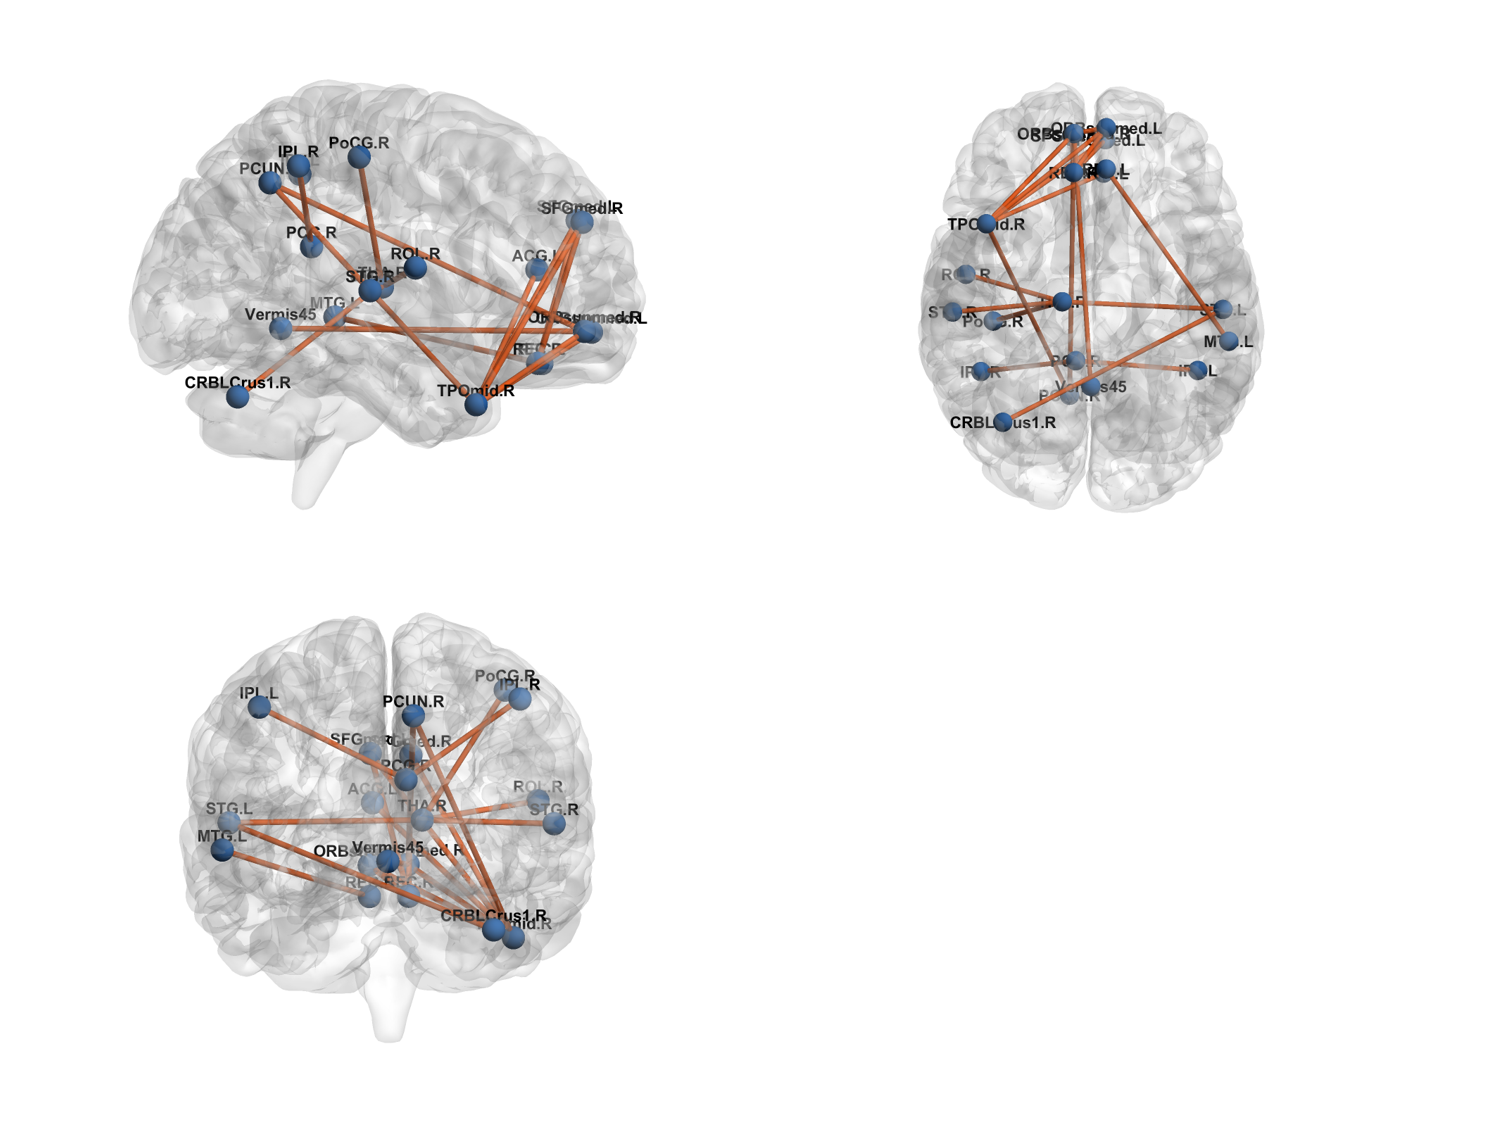
\includegraphics[width=0.8\textwidth]{imgs/brain.png}
	\caption{Projection of the top 20 most discriminative functional connections in the brain}
	\label{fig3}
\end{figure*} 

To identify the most relevant features associated with the onset of autism, we ranked the top 100 features for each window and tallied the number of times each feature appeared across all rankings. We selected the 30 features with the highest number of occurrences for further analysis and presentation. The corresponding brain regions and their distribution across brain hemispheres are summarized in Table \ref{Table6}, and the brain projection map is depicted in \figref{fig3}.

Our analysis revealed that the superior frontal gyrus and middle temporal gyrus had a significant impact on ASD. Regarding functional connectivity, the Cingulum Ant and TemporaI Pole Mid were the only functional connections that appeared in all windows. Connections between Frontal Sup Medial and Rectus, as well as Frontal Mid 0rb and Precuneus, were present in almost all windows. Additionally, the relationship between the thalamus and temporal lobe was frequently observed and noteworthy. Similar results have been obtained in previous studies(\cite{wang2021autistic},\cite{monk2009abnormalities},\cite{xu2020specific}).

\begin{table*}[]
	\tabcolsep=1cm
	\caption{10 brain connections most likely to cause ASD}\label{Table6}
	\begin{tabular*}{\tblwidth}{@{}ccccc@{}}
		\toprule
\textbf{ID} & \textbf{ROIs}      & \textbf{\textbf{Hemisphere}} & \textbf{\textbf{ROIs}} & \textbf{\textbf{\textbf{\textbf{Hemisphere}}}} \\ \midrule
1           & Cingulum Ant       & L                            & TemporaI Pole Mid      & R                                              \\
2           & Frontal Mid 0rb    & R                            & Precuneus              & R                                              \\
3           & Frontal Sup MediaI & L                            & Rectus                 & R                                              \\
4           & Postcentral        & R                            & Thalamus               & R                                              \\
5           & TemporaI Sup       & L                            & Thalamus               & R                                              \\
6           & Frontal Mid 0rb    & L                            & Frontal Mid 0rb        & R                                              \\
7           & FrontaI Sup Medial & R                            & Rectus                 & R                                              \\
8           & FrontaI Sup Medial & R                            & TemporaI Pole Mid      & R                                              \\
9           & Thalamus           & R                            & TemporaI Sup           & R                                              \\
10          & FrontaI Sup Medial & L                            & TemporaI PoIe Mid      & R                                              \\
11          & Frontal Mid 0rb    & L                            & Rectus                 & R                                              \\
12          & RoIandic Oper      & R                            & Thalamus               & R                                              \\
13          & Frontal Mid 0rb    & R                            & TemporaI Pole Mid      & R                                              \\
14          & Rectus             & L                            & TemporaI Mid           & L                                              \\
15          & Precuneus          & R                            & TemporaI PoIe Mid      & R                                              \\
16          & Cingulum Post      & R                            & Parietal Inf           & R                                              \\
17          & Frontal Mid 0rb    & L                            & TemporaI PoIe Mid      & R                                              \\
18          & ~TemporaI Sup      & L                            & Cerebelum Crus 1       & R                                              \\
19          & Parietal Inf       & L                            & Cingulum Post          & R                                              \\
20          & Precuneus          & L                            & Frontal Mid 0rb        & R   \\
		\bottomrule
	\end{tabular*}
\end{table*}

\section{Discussion}
In this paper, we employed sliding windows to partition the time series into multiple overlapping and independent windows. For each window, a functional connectivity vector was generated using the Pearson correlation coefficient, and these vectors were combined to generate dFC. Compared to the widely used static FC, dFC captures fluctuations in the temporal dimension of the BOLD signal. However, it also exacerbates the conflict between small sample size and high dimensionality, making feature extraction crucial to similar research.

We employed Kendall's rank correlation coefficient for feature extraction, which enabled us to select features with high discriminative power without changing the raw data. All feature selection was performed prior to model training, significantly reducing the time required for training. Our results demonstrated that the model achieved the highest performance when 1024 features are chosen for training, highlighting the sparsity of the brain functional connectivity network and emphasizing the importance of feature extraction in relevant research. Selecting more discriminative features is a crucial prerequisite for achieving excellent model performance.

To address the self-attention mechanism's inability to model temporal order, we incorporated positional encoding into the input data. This encoding method accurately represents the input order of the windows without increasing the model's parameters, making it easier for the model to capture variations in nearby windows. The multi-head self-attention mechanism is exceptional at gaining global information, with the multiple heads enabling the model to acquire knowledge from several subspaces. We also employ feedforward neural networks to obtain feature combinations in higher-dimensional spaces and eliminate feature combinations with low discrimination by recovering the preceding dimension. Residual networks help decrease gradient disappearance and accelerate model training. Our model achieves an average accuracy of 76.22\% and an AUC of 0.8132 in ten-fold cross-validation. Furthermore, inter-site cross-validation demonstrated the model's strong generalizability, achieving an average accuracy of 76.71\% and an AUC of 0.7955. In our studies, the model worked optimally at $H$=6, demonstrating that the brain functional connectivity network includes a plethora of information. Future studies should place a greater emphasis on extracting the data's abundant information, such as utilizing HOFC to define the correlation of correlations between brain regions.

Using the Kendall feature ranking, we identified the 20 functional connections most likely to be associated with ASD. The superior frontal gyrus and middle temporal gyrus were found to be the most connected regions contributing to the prevalence of ASD. Connections between the cingulum Ant and TemporaI Pole Mid, Frontal Sup Medial and Rectus, Frontal Mid 0rb, and Precuneus were present in the majority of windows. Additionally, the relationship between the thalamus and temporal region was bound to be significant. These findings provide valuable insights for future studies on the pathophysiology of ASD.
\section{Conclusion}
In this study, we proposed a self-attention mechanism-based method for diagnosing autism. We utilized sliding windows to construct dynamic functional connectivity from raw data and applied Kendall rank correlation coefficients for feature selection. By stacking multi-head self-attention layers and adding a feed-forward neural network structure, the model was able to capture correlations between time windows and extract higher-order spatial features, resulting in outstanding results in discriminating ASD. Our feature ranking analysis identified the superior frontal gyrus and middle temporal gyrus as having the most significant impact on ASD. Our model contributes to the field of deep learning for mental disorder diagnosis and research on autism pathology.
% To print the credit authorship contribution details
%\printcredits

%% Loading bibliography style file
%\bibliographystyle{model1-num-names}
\bibliographystyle{cas-model2-names}

% Loading bibliography database
\bibliography{ref/refs.bib}

% Biography
%\bio{}
% Here goes the biography details.
%\endbio

%\bio{pic1}
% Here goes the biography details.
%\endbio

\end{document}

